% Source: https://github.com/mtrimoska/Tikz_figures_from_my_Thesis/blob/main/6_1/6_1.tex

\documentclass[a4paper,12pt]{report}
\usepackage[utf8]{inputenc}


\usepackage{tikz}
\usetikzlibrary{calc}
\usepackage{subcaption}

\begin{document}

\thispagestyle{empty}

\begin{figure}[h!]
		\centering
		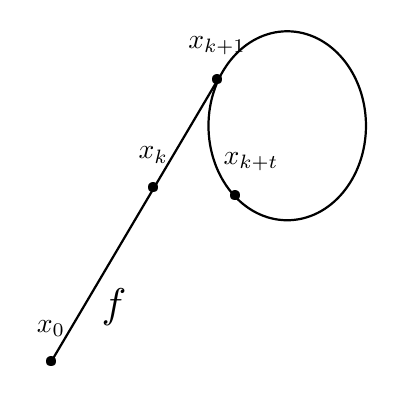
\begin{tikzpicture}
		
		\node[scale=1.5] at (-2.2,-2.3) {$f$};
		\draw [thick] (0,0) ellipse (1cm and 1.2cm);
		\draw [thick] (-3,-3) -- (-0.89,0.57);
		\node[label={$x_0$},scale=1] (1) at (-3,-3) {\textbullet};
		\node[label={$x_{k+1}$},scale=1] (2) at (-0.89,0.57) {\textbullet};
		\node[label={$x_{k}$},scale=1] (3) at (-1.7,-0.8) {\textbullet};
		\node[label={[shift={(0.2,0)}]$x_{k+t}$},scale=1] (4) at (-0.66,-0.9) {\textbullet};
	
		\end{tikzpicture}
		\caption{Pollard's rho walk.}
		\label{fig:rho}
	\end{figure}


\end{document}